\documentclass{zkdl-presentation-template}

% -- Auxiliary Packages --
\usepackage{pgffor}
\usepackage{bbm}

% -- Algorithms --
\usepackage[
    titlenumbered,
    linesnumbered,
    ruled
]{algorithm2e}
\SetKwInOut{Input}{Input}
\SetKwInOut{Output}{Output}
\SetKwInOut{Return}{Return}

% --- Ticks and crosses ---
\usepackage{pifont} % http://ctan.org/pkg/pifont
\newcommand{\cmark}{\textcolor{green!65!black}{\ding{51}}}%
\newcommand{\xmark}{\textcolor{red!80!black}{\ding{55}}}%

% --- Tikz ---
\usetikzlibrary{tikzmark, backgrounds, shapes.geometric, arrows.meta, positioning, fit}

% --- Code settings ---
% Required package for syntax highlighting
% You must compile your LaTeX document with the -shell-escape flag
% For example: pdflatex -shell-escape your_document.tex
\usepackage{minted}

% --- Optional: Global settings for the minted environment ---
% This makes the code block look nice on a slide
\setminted{
    frame=lines,          % Puts a thin border around the code
    framesep=2mm,         % Adds some padding inside the border
    baselinestretch=1.1,  % Improves line spacing for readability
    fontsize=\scriptsize, % Adjusts font size to fit more code
    linenos,              % Adds line numbers
    breaklines            % Automatically breaks long lines
}

% --- Nice random sample sign ---
\newcommand\leftarrowS{\leftarrow\joinrel\smalldollar}
\newcommand\rightarrowS{\smalldollar\joinrel\rightarrow}

\makeatletter
\newcommand{\smalldollar}{\mathrel{\mathpalette\small@dollar\relax}}
\newcommand{\small@dollar}[2]{%
  \vcenter{\hbox{%
    $#1\textnormal{\fontsize{0.7\dimexpr\f@size pt}{0}\selectfont\$}$%
  }}%
}
\makeatother

% --- Title Page Info ---
\title[UltraGroth]{UltraGroth: Interactive Groth16}
\author{Dmytro Zakharov \\ Distributed Lab}
\date{August 29, 2025}
\homepage{distributedlab.com/}
\github{rarimo/ultragroth}

\begin{document}
    \frame {
        \tikz [remember picture,overlay]
        \node at
            ([yshift=3.0cm,xshift=-3.0cm]current page.south east) 
            %or: (current page.center)
            {
\includegraphics[width=100pt]{logo.png}};
        \titlepage
    }

	\section{Why we should care?}

    \begin{frame}{Range Checks}
        \begin{block}{Problem}
            Write a circuit that checks whether $x$ is a $128$-bit integer.
        \end{block}

        Current R1CS (and, consequently, Circom's) approach is to 
        conduct the following steps:
        \begin{itemize}
            \item Find bit decomposition of $x$ off-circuit: say, $x=\sum_{i=0}^{127}x_i2^i$.
            \item Check that $x_i \in \{0,1\}$: impose $128$ constraints $x_i(1-x_i)=0$.
        \end{itemize}

        \textbf{Result:} 128 constraints per \textit{128-bit range check}.

        \begin{alertblock}{Question}
            Suppose one needs to conduct $10000$ such range checks. How many 
            constraints does one need to implement this?
        \end{alertblock}
        
        Using quite unsophisticated math, $128 \times 10000 = \textcolor{red!70!black}{\textbf{1.28\,\text{mln}}}$.
    \end{frame}

    \begin{frame}{Better range checks}
        Using lookup checks, we can implement the same logic in just
        $\approx\textcolor{green!70!black}{100\text{k}}$ constraints! Here is
        how.

        \textbf{Assumption.} Assume we can check whether the given signal $s$ is
        the $w$-bit integer in \textit{a single constraint}. But this requires 
        a \textit{one-time} cost of $2^w$ constraints. How does it help us?

        Suppose we use $w := 16$. Then, our algorithm proceeds as follows:
        \begin{itemize}
            \item We pay $2^{16} \approx 65.5\text{k}$ for a one-time commitment.
            \item We find $w$-width decomposition of $x$: say, $x = \sum_{i=0}^{7}x_i2^{wi}$.
            \item We check whether $x_i$ is a $16$-bit integer. Since we have $8$ chunks,
            this costs $8$ constraints.
        \end{itemize}

        \textbf{Result:} We pay $65.5\text{k}$ constraints once and then every 
        128-bit range checks costs only $8$ constraints instead of $128$!
    \end{frame}

    \begin{frame}{Illustration}
        Let us illustrate this visually for a $16$-bit range check over
        $x$!

        \vspace{10px}

        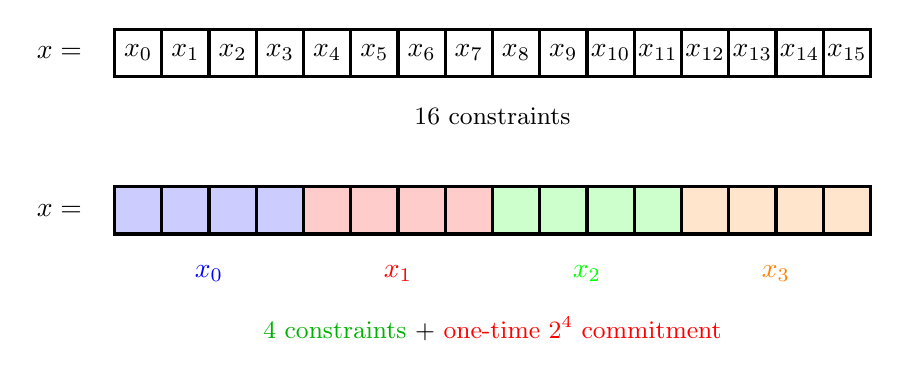
\begin{tikzpicture}[
            % Style for the bit squares, now smaller
            bit/.style={draw, very thick, minimum size=0.6cm, outer sep=0},
            % Style for the labels below the rows
            info/.style={font=\small}
        ]

        % --- First line: 16 individual bits ---
        \node at (-1, 2.0) {$x=$};
        % Draw the 16 squares and labels separately to ensure constant box size
        \foreach \i in {0,...,15} {
            % Draw the box first
            \node[bit] at (\i*0.6, 2.0) {};
            % Then place the label at the same coordinate
            \node at (\i*0.6, 2.0) {$x_{\i}$};
        }
        % Add the text below the row, centered
        \node[info] at (7.5*0.6, 1.2) {16 constraints};


        % --- Second line: 4 chunks of 4 bits ---
        \node at (-1, 0) {$x=$};
        % Draw the 4 highlighted chunks with different gentle colors and their labels
        \foreach \i/\chunkcolor/\textcolor in {0/blue!20/blue, 1/red!20/red, 2/green!20/green, 3/orange!20/orange} {
            % Draw the colored rectangle for the chunk
            \fill[\chunkcolor] (\i*4*0.6 - 0.3, -0.3) rectangle (\i*4*0.6 + 4*0.6 - 0.3, 0.3);
            % Add the chunk label below with corresponding color
            \node[text=\textcolor, font=\bfseries] at (\i*4*0.6 + 1.5*0.6, -0.8) {$x_{\i}$};
        }
        % Draw the 16 squares on top (without labels)
        \foreach \i in {0,...,15} {
            \node[bit] at (\i*0.6, 0) {};
        }
        % Draw vertical lines to separate the chunks
        \foreach \i in {1,2,3} {
            \draw[thick] (\i*4*0.6 - 0.3, -0.3) -- (\i*4*0.6 - 0.3, 0.3);
        }
        % Add the text below the row, centered
        \node[info, text width=10cm, align=center] at (7.5*0.6, -1.5) {\textcolor{green!70!black}{4 constraints} + \textcolor{red}{one-time $2^4$ commitment}};

        \end{tikzpicture}

        \textbf{Example:} $10000$ such range checks would cost $16 \times 10000
        = 160\text{k}$ constraints for a regular R1CS while $2^4 + 4 \times
        10000 \approx 40\text{k}$ constraints over ZK system with lookups.
    \end{frame}

    \begin{frame}{Applications}
        \begin{itemize}
            \item Wrappings of non-native ZKP verifications: e.g., zk-STARKs, 
            sumcheck-based approaches.
            \item Non-native field arithmetic: e.g., optimized ECDSA
            verification for Rarimo passport verification.
            \item And surely, zero-knowledge Machine Learning --- Bionetta.
        \end{itemize}
        \begin{figure}
            \centering
            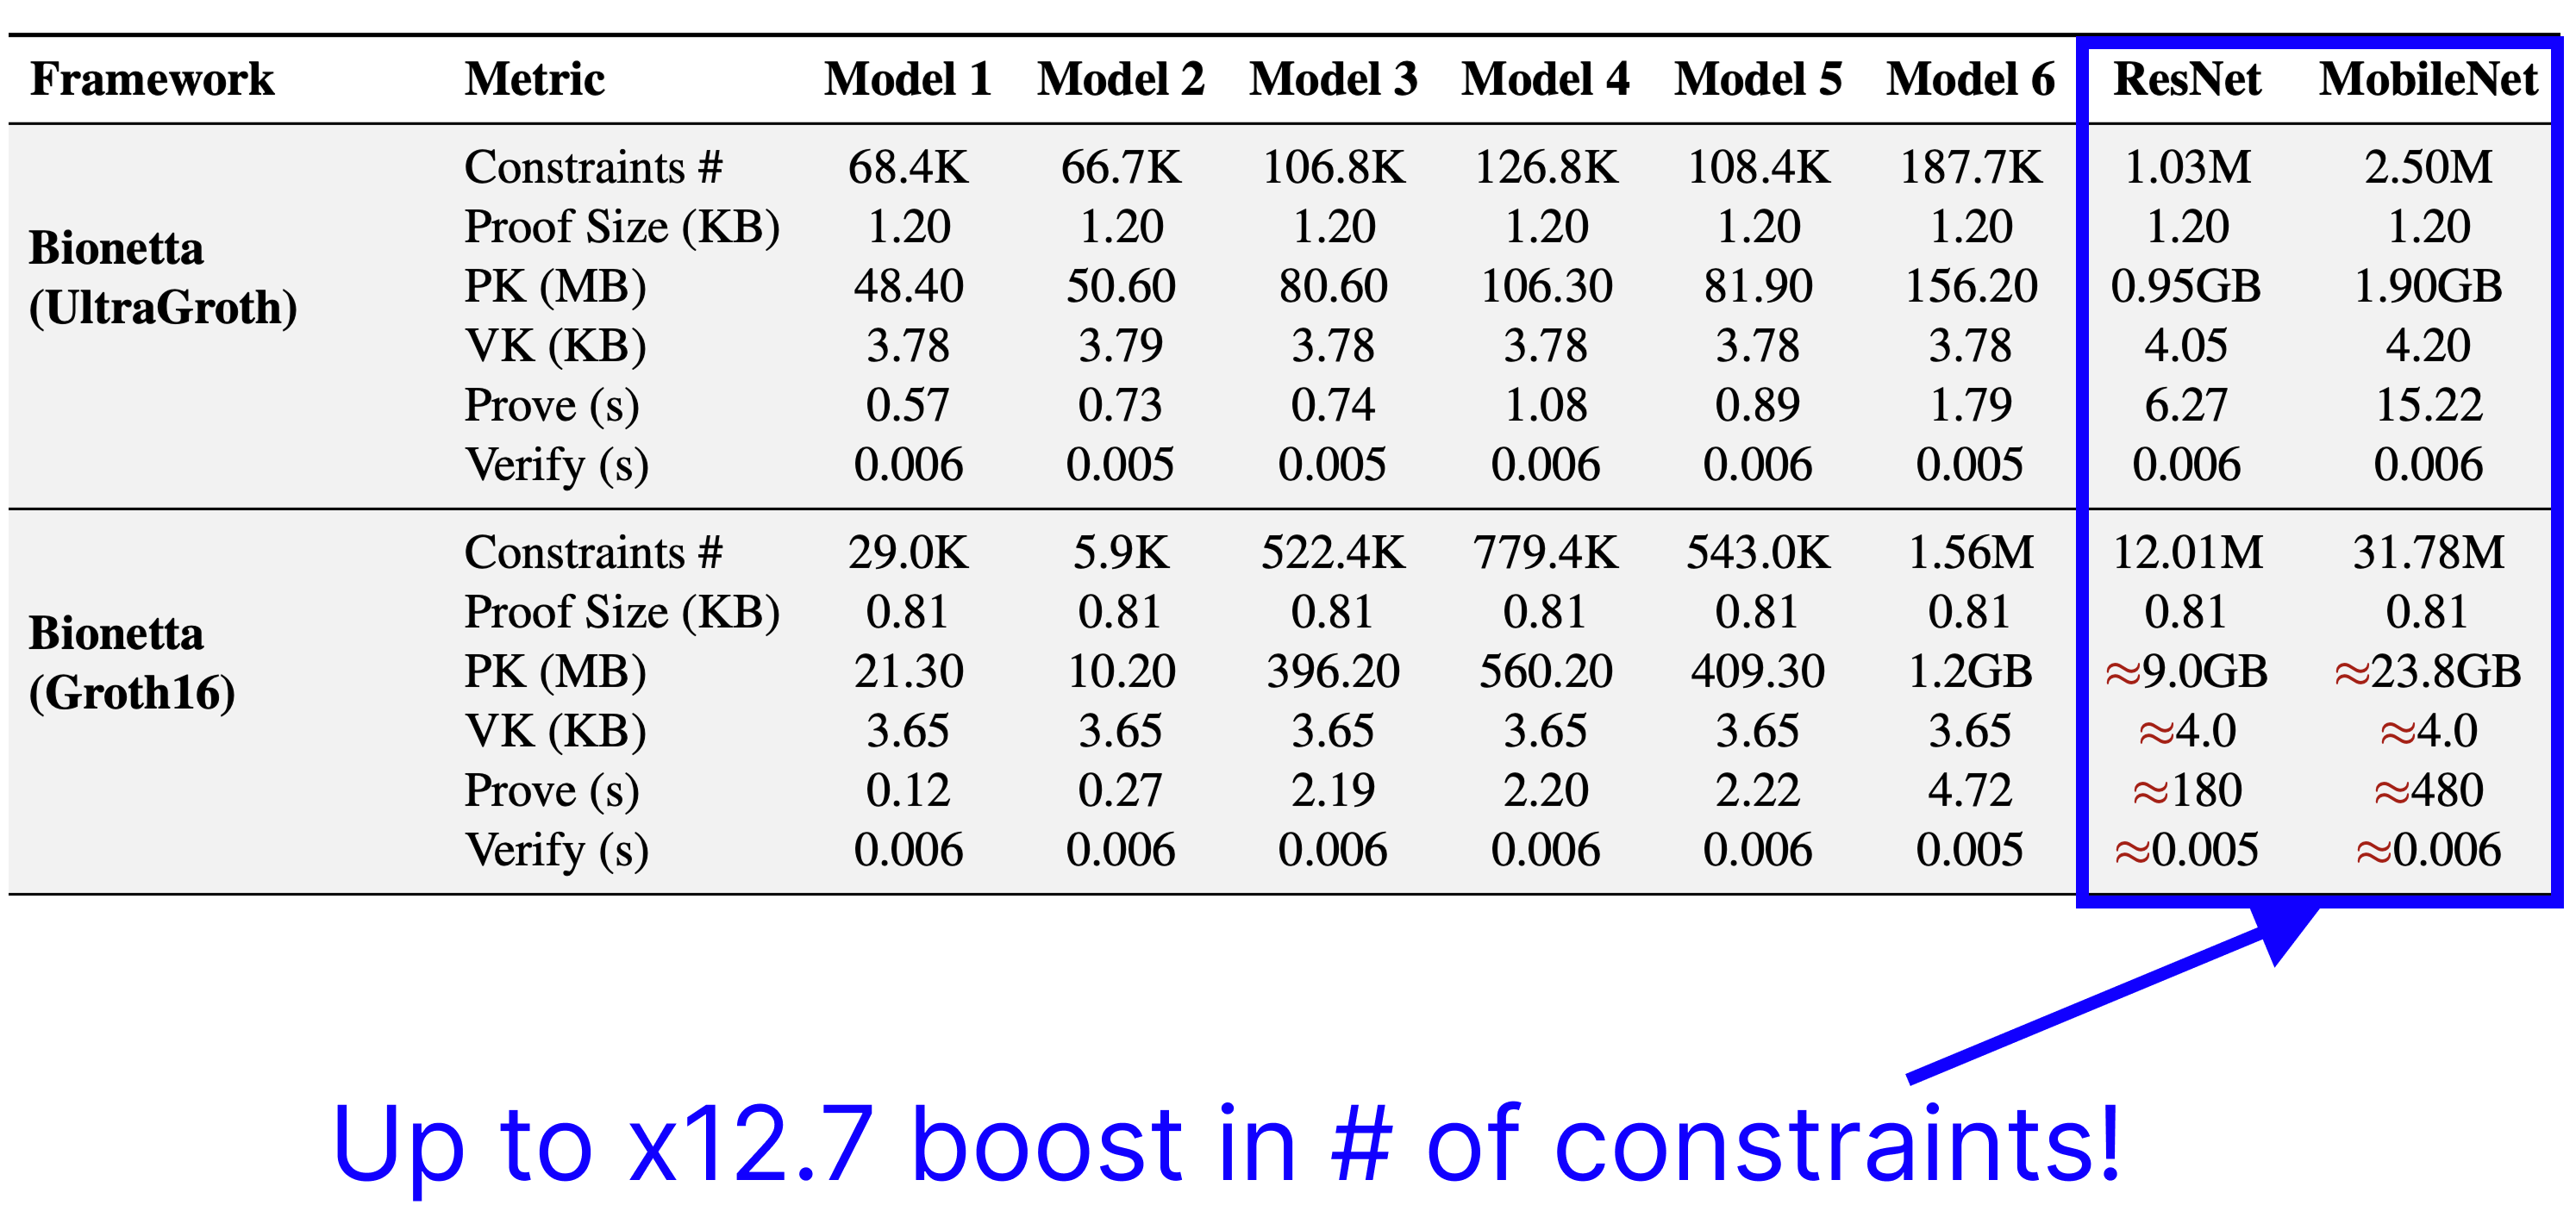
\includegraphics[width=0.95\textwidth]{images/benchmark.png}
        \end{figure}
    \end{frame}

    \begin{frame}{How to actually implement?}
        \textcolor{blue!70!black}{\textbf{Surprising result}}: if the circuit
        consists of $L$ range-checks, each costing $b$ constraints, using lookup
        protocol, you can reduce \textcolor{blue!70!black}{$\mathcal{O}(n)$}
        constraints ($n=Lb$) down to
        \textcolor{blue!70!black}{$\mathcal{O}(n/\log n)$}.

        \textcolor{blue!70!black}{\textbf{Key question:}} \textit{how do we
        implement it \textbf{in Groth16?}} Since PlonK and SumCheck already have
        them! (see plookup+logup).

        \begin{theorem}[Some stuff from ZKDL Camp]
            The inclusion check $\{z_i\}_{i \in [n]} \subseteq \{t_i\}_{i \in
            [v]}$ is satisfied if and only if there exists the set of
            multiplicities $\{\mu_i\}_{i \in [v]}$ where $\mu_i = \#\{j \in [n]:
            z_j = t_i\}$ such that for $\gamma \leftarrowS \mathbb{F}$:
            \begin{equation*}
                \sum_{i \in [n]} \frac{1}{\gamma + z_i} = \sum_{i \in [v]} \frac{\mu_i}{\gamma + t_i}
            \end{equation*}
        \end{theorem}

        \textit{High-level idea:} We can: (1) compute $\{\mu_i\}_{i \in [v]}$
        off-circuit, (2) write circuit in $n+2v$ constraints,
        \textcolor{red!70!black}{given $\gamma$ signal is passed randomly}.
    \end{frame}

\begin{frame}[fragile]
    \frametitle{Circom-like Implementation}

    \begin{minted}{javascript}
    signal input t[M];         // The lookup table
    signal random input gamma; // Random challenge value
    signal input z[N];         // The array of values to check

    var sum_z, sum_t = 0;
    for (var i = 0; i < N; i++) {
        inv_z[i] <== 1 / (z[i] + gamma);
        sum_z += inv_z[i]; // Compute the left-hand side
    }

    for (var j = 0; j < M; j++) {
        mu[j] <-- 0; // Compute the multiplicities off-circuit
        for (var k = 0; k < N; k++) {
            mu[j] += (t[j] == z[k]);
        }
        inv_t[i] <== mu[j] / (t[j] + gamma);
        sum_t += int_v[i]; // Compute the right-hand side
    }

    sum_z === sum_t; // Check both sides are equal
    \end{minted}
\end{frame}

\begin{frame}[fragile]
    \frametitle{Problem}

    \begin{minted}[
        highlightlines={2},
        highlightcolor={red!25}
    ]{javascript}
    signal input t[M];         // The lookup table
    signal random input gamma; // Random challenge value
    signal input z[N];         // The array of values to check

    var sum_z, sum_t = 0;
    for (var i = 0; i < N; i++) {
        inv_z[i] <== 1 / (z[i] + gamma);
        sum_z += inv_z[i]; // Compute the left-hand side
    }

    for (var j = 0; j < M; j++) {
        mu[j] <-- 0; // Compute the multiplicities off-circuit
        for (var k = 0; k < N; k++) {
            mu[j] += (t[j] == z[k]);
        }
        inv_t[i] <== mu[j] / (t[j] + gamma);
        sum_t += int_t[i]; // Compute the right-hand side
    }

    sum_z === sum_t; // Check both sides are equal
    \end{minted}
\end{frame}

\section{UltraGroth Explained}

\begin{frame}{Some Historical Notes}
    \begin{itemize}
        \item First paper on this problem is
        \textcolor{green!70!black}{``\textsf{MIRAGE}: Succinct Arguments for
        Randomized Algorithms with Applications to Universal zk-SNARKs''},
        published in \textcolor{blue!70!black}{2020}.
        \item Unaware of this protocol, in \textcolor{blue!70!black}{2023} Lev
        Soukhanov published the post on
        \textcolor{green!70!black}{\textbf{UltraGroth}}, where he invented
        \textit{multi-round} MIRAGE.
        \item Likely, unaware of Lev Soukhanov's blog, Alex Ozdemir, Evan
        Laufer, Dan Boneh published \textcolor{green!70!black}{``Volatile and
        persistent memory for zkSNARKs via algebraic interactive proofs''} paper
        in \textcolor{blue!70!black}{2025}.
        \item Well... Their construction, called MIRAGE+, is exactly an
        \textcolor{green!70!black}{\textbf{UltraGroth}}, published back in 2023.
    \end{itemize}

    \begin{block}{One important consequence}
        The protocol is \textbf{safe}. It is sound and zero-knowledge! And it is
        now proven in \textbf{three} different independent papers.
    \end{block}
\end{frame}

\begin{frame}{UltraGroth Performance}
    Now, let us recap the \textcolor{green!70!black}{\textbf{Groth16} performance} over
    the circuit of size $n$ and statement size $\ell$.
    \begin{itemize}
        \item \textbf{Prover work}: MSM of size $\mathcal{O}(n)$ over
        $\mathbb{G}_1$ and $\mathbb{G}_2$.
        \item \textbf{Proof size:} $2\mathbb{G}_1+\mathbb{G}_2$.
        \item \textbf{Verifier work:} 3 pairings + $\mathcal{O}(\ell)$
        $\mathbb{G}_1$ exps.
    \end{itemize}

    \textcolor{blue!70!black}{\textbf{UltraGroth} performance} in turn:
    \begin{itemize}
        \item \textbf{Prover work}: MSM of size
        $\mathcal{O}(\textcolor{blue!70!black}{n/\log n})$ over $\mathbb{G}_1$
        and $\mathbb{G}_2$.
        \item \textbf{Proof size:}
        $\textcolor{blue!70!black}{3}\mathbb{G}_1+\mathbb{G}_2$ (additional 64
        bytes).
        \item \textbf{Verifier work:} \textcolor{blue!70!black}{4} pairings +
        $\mathcal{O}(\ell)$ $\mathbb{G}_1$ exps + \textcolor{blue!70!black}{1
        hashing}.
    \end{itemize}
\end{frame}

\begin{frame}{UltraGroth Overall Idea}
    \textbf{Problem:} Compared to PlonK or SumCheck, \textit{Groth16} itself is
    not derived from the interactive protocol (via Fiat-Shamir).

    \textbf{Recap:} Proof in Groth16 consists of three points $g_1^{a(\tau)}$,
    $g_1^{c(\tau)}$, $g_2^{b(\tau)}$:
    \begin{gather*}
        a(X) = \alpha + \sum_{i \in [n]}z_i\ell_i(X) + r\delta, \quad b(X) = \beta + \sum_{i \in [n]}z_ir_i(X) + s\delta, \\
        c(X) = \delta^{-1}\left(\sum_{i \in \mathcal{I}_W} z_i\zeta_i(X)+h(X)t(X)\right) + a(X)s + b(X)r - rs\delta.    
    \end{gather*}

     The \textbf{verification equation} is:
    \begin{equation*}
        e(\pi_A,\pi_B) = e(g_1^{\alpha},g_2^{\beta})\cdot e(g_1^{i(\tau)},g_2^{\gamma})\cdot e(\pi_C,g_2^{\delta}).
    \end{equation*}
    for $\pi_A = g_1^{a(\tau)}$, $\pi_C = g_1^{c(\tau)}$, $\pi_B =
    g_2^{b(\tau)}$, $i(X)$ is a polynomial derived from the public statement.
\end{frame}

\begin{frame}{UltraGroth Overall Idea}
    \begin{itemize}
        \item Do not touch $a(X)$ and $b(X)$.
        \item Split R1CS into two rounds:
        \textcolor{blue!70!black}{\textit{round 0}} computes the circuit without
        lookup check, \textcolor{green!70!black}{\textit{round 1}} imposes
        lookup check.
        \item Split $c(X)$ into \textcolor{blue!70!black}{$c_0(X)$} and
        \textcolor{green!70!black}{$c_1(X)$}. 
        \item $c_0(X)$ is derived from \textcolor{blue!70!black}{\textit{round
        0}}'s witness. 
        \item Form point $\textcolor{blue!70!black}{\pi_C^{\langle 0 \rangle}}
        \gets
        g_1^{\textcolor{blue!70!black}{\textcolor{blue!70!black}{c_0(\tau)}}}$
        and sample randomness $\gamma \gets
        \mathcal{H}(\textcolor{blue!70!black}{\pi_C^{\langle 0 \rangle}})$.
        \item Compute witness for \textcolor{green!70!black}{\textit{round 1}} using $\gamma$,
        form \textcolor{green!70!black}{$c_1(X)$} and thus compute
        $\textcolor{green!70!black}{\pi_C^{\langle 1 \rangle}} \gets
        g_1^{\textcolor{green!70!black}{c_1(\tau)}}$.
        \item Output proof as $\pi \gets (\pi_A, \textcolor{blue!70!black}{\pi_C^{\langle
        0 \rangle}}, \textcolor{green!70!black}{\pi_C^{\langle 1 \rangle}}, \pi_B)$.
    \end{itemize}

    The \textbf{verification equation} is:
    \begin{equation*}
        e(\pi_A,\pi_B) = e(g_1^{\alpha},g_2^{\beta})\cdot e(g_1^{i(\tau)},g_2^{\gamma})\cdot \textcolor{blue!70!black}{e(\pi_C^{\langle 0 \rangle},g_2^{\delta_0}) \cdot e(\pi_C^{\langle 1 \rangle},g_2^{\delta})}.
    \end{equation*}

    \textbf{Note:} This construction can be easily generalized for $d>1$ rounds.
\end{frame}

\begin{frame}{Our Contribution}
    \begin{itemize}
        \item Implemented a single-round UltraGroth (essentially, a Mirage
        protocol). Credits to Artem Sdobnov, Vitalii Volovyk, Yevhenii 
        Sekhin, and Illia Dovgopoly.
        \begin{itemize}
            \item Forked \texttt{rapidsnark}.
            \item Forked \texttt{snarkjs} for witness export/verify functions
            and smart-contract autogeneration.
            \item Thanks to Ivan Lele, we even have a Swift SDK for that!
        \end{itemize}
        \item Proved completeness, soundness, and zero-knowledge for general
        $d$-round UltraGroth. Formalized everything properly.
        \item Applied UltraGroth to Bionetta and obtained incredible results.
    \end{itemize}
\end{frame}

    \begin{frame}[plain]
        \centering
        \LARGE
        \textbf{Any Questions?} \\
        
        \vspace{0.2cm} \Huge \ding{170} \large \\
        
        \vspace{1cm}
  
        \href{https://distributedlab.com/}{\raisebox{-.1em}{\hspace{.025em}\faIcon{globe}}\hspace{.325em}distributedlab.com} \\
  
        \href{https://github.com/rarimo/ultragroth}{\raisebox{-.1em}{\hspace{.025em}\faIcon{github}}\hspace{.325em}github.com/rarimo/ultragroth}
        
        \begin{center}
            
\includegraphics[width=0.25\textwidth]{logo.png}
        \end{center}
    \end{frame}
\end{document}